\documentclass[11pt]{amsart}
\usepackage{geometry}                % See geometry.pdf to learn the layout options. There are lots.
\geometry{letterpaper}                   % ... or a4paper or a5paper or ... 
%\geometry{landscape}                % Activate for for rotated page geometry
\usepackage[parfill]{parskip}    % Activate to begin paragraphs with an empty line rather than an indent
\usepackage{graphicx}
\usepackage{amssymb}
\usepackage{epstopdf}
\DeclareGraphicsRule{.tif}{png}{.png}{`convert #1 `dirname #1`/`basename #1 .tif`.png}
\usepackage{amsfonts,amsmath,amsthm,amsbsy,latexsym,amssymb,graphicx,booktabs,multicol,color,fullpage}
\usepackage{mathabx,dashrule}
\usepackage{pgf,tikz}
\usepackage{pgfplots}
\usepackage{graphicx}
\usepackage{wrapfig}
\usepackage[mathscr]{eucal}
\usepackage{multicol}
\usepackage{arydshln}
\usepackage{verbatim}
\usepackage{xcolor}
\newcommand{\subf}[2]{%
  {\small\begin{tabular}[t]{@{}c@{}}
  #1\\#2
  \end{tabular}}%
}



\title{Three Stabilization Schemes for an Application of Fourier Continuation Approximations}
\author{Melanie Vining \\ Integrated and Applied Mathematics \\University of New Hampshire}
%\date{}       

\begin{document}
\maketitle
\newpage
$N$ - number of points on grid\\
$M$ - number of modes used\\
$n$ - integer index\\


\newpage


\section{Introduction}
Function approximation has long been associated with numjerical solutions of differential equations.  In particular, Fourier Series are in common use for solving differential equations on equispaced grids. However, when approximating a non-periodic function with a (truncated, discrete) Fourier Series, it is possible to get error at the endpoints in the form of Gibbs' phenomenon, and when solving differential equations this error can propagate and destroy the accuracy across the grid for the entire solution.  \\
To approximate non-periodic functions with the end goal of using Fourier Series methods (fast Fourier transforms with numerical differentiation) for any application, but of particular interest to this dissertation for finding numerical solutions of differential equations, one method that can be employed is to instead use Fourier Continuation approximations, also known as Fourier extensions, first introduced in [sources].  Analysis of these continuation approximations shows that accuracy is preserved in conjunction with their immediate use in Fourier Series [sources]. As a result of the high accuracy afforded by Fourier continuations, further schemes have been implemented to directly apply Fourier continuation approximations to the solution of differential equations, and in particular partial differential equations. \\
Using the idea of ADI methods as a guide [source], Fourier continuation approximations can be implemented in what is referred to as the FC-AD method [sources].  This is used to numerically solve parabolic or hyperbolic PDEs, like the 2-D heat equation or the 2-D wave equation.  Use of this method results in a 2nd order differential equation which is solved using Fourier Continuation approximations.  The result is a highly accurate and stable scheme [source]. 

Other accurate, stable schemes for numerically solving PDEs include ** ** **.  However, each of these schemes is limited in their accuracy 


\subsection{Function Approximation and Ordinary Differential Equation Solutions} 
 It is often useful to approximate a function instead of using its original representation. The representation of the function in the terms of another basis can allow for analysis of the function as it behaves with respect to properties of the basis. The properties of the basis in a given situation may have benefits in application that the function itself may not exhibit.  
 
 Given a basis $\{g_0$,$g_1$,$\ldots$, $g_{n1-}\}$, a function $f$ can be approximated as 
 \begin{equation*}
 f=c_0g_0+c_1g_1+\ldots+c_ng_{n-1}.
 \end{equation*}  
 If the function has been discretized on a grid, then the basis, also discretized, can still approximate the function.  In this case, the coefficients $c_0,\ldots c_{n-1}$ can be found by a QR-factorization. If the basis $g_0 \ldots g_{n-1}$ is an orthonormal basis, to find the coefficients to approximate $f$, first, matrices are create.  Let $G$ be the matrix whose columns are the discretized values of the basis, 
 \begin{equation*}
 G=\begin{bmatrix}
 \vline & \vline & \vline &  & \vline \\
 g_0 & g_1 & g_2 & \ldots & g_{n-1} \\
 \vline & \vline & \vline &  & \vline 
 \end{bmatrix}.
 \end{equation*}
 This creates the matrix equation
 \begin{equation}
 G\vec{c}=f
 \end{equation}
 where $\vec{c}$ are the coefficients in ascending order.  
 The solution is found by inverting the matrix $G$.  Computationally, this is done effectively with a QR-factorization.  This method is preferred over other methods of inversion not only because of its numerical stability but also because of its direct portability to a least-squares solver in the event of a projection from the space of the function into the space of the basis.  \\ 
 Function approximation can be particularly useful when approximating solutions to differential equations for which the analytic solutions are unreachable or otherwise impractical.  
 In the example of even a linear second order differential equation like
 \begin{equation*}
 a\dfrac{d^2u}{dx^2} + b\dfrac{du}{dx}+cu = f
 \end{equation*}
  if the forcing function $f$ is in any way complicated, the solution $u$ may not be able to be expressed explicitly. 
  One way to approximate the solution is to approximate the expression obtained by using analytical methods to solve (e.g. if solving using variation of parameters, and approximating the resulting integral), but another way to approximate the solution is to discretize the differential equation and solve using an appropriate numerical method. 
The choice of how to approximate the differential operator comes down to (generally) 3 methods: finite difference methods, spectral methods, and finite element methods (of which finite difference methods technically belong, but whose application reaches beyond finite difference methods). 
Finite difference methods are simple to implement and yield stable results as long as certain conditions are met.
  
  
 
 
 
 
 \subsection{Fourier series} 
 
 
 A function $f$ is called periodic if for some $T>0$ and for all $x$ in the domain of $f$, $f(x)=f(x+T)$.
 Note that any function that has period $T$ also has period $nT$, $n \in \mathbb{Z}^{+}$.
 Consider the functions $\cos(nx)$ and $\sin(nx)$, $n\in \mathbb{Z}^{+}$.  Each function of this form has a period $\dfrac{2\pi}{n}$, and thus also has a period of $2\pi $. 
Thus the sum $c+\sum_{n=1}^{\infty} a_n \cos(nx) + b_n \sin(nx)$, if it converges, represents a function that is periodic of with period $2\pi$. \\
Given a function $f(x)$ that is periodic with period $2\pi$, is it guaranteed to have a series representation of the form above? 
Suppose there is, and that
\begin{equation}
\label{eqn:Fourier}
f(x)=\dfrac{a_0}{2}+\sum_{k=1}^{\infty} a_k \cos(kx)+b_k \sin(kx).
\end{equation}
Integrating from $-\pi$ to $\pi$ (over a full period) yields
\begin{equation}
\int_{-\pi}^{\pi}f(x)dx=\int_{-\pi}^{\pi} \frac{a_0}{2} + \int_{-\pi}^{\pi} \sum_{k=1}^{\infty} a_k \cos(kx)+b_k \sin(kx)dx
\end{equation}
Assuming that the sum can be integrated term-by-term (that the sum converges absolutely) gives that
\begin{equation}
\int_{-\pi}^{\pi}f(x)dx=\int_{-\pi}^{\pi} \frac{a_0}{2} + \sum_{k=1}^{\infty}\int_{-\pi}^{\pi}  a_k \cos(kx)dx+ \sum_{k=1}^{\infty}\int_{-\pi}^{\pi} b_k \sin(kx)dx
\end{equation}
so 
\begin{equation}
\int_{-\pi}^{\pi} f(x)dx= \pi a_0
\end{equation}

and the first coefficient\begin{equation} a_0=\dfrac{1}{\pi}\displaystyle \int_{-\pi}^{\pi} f(x)dx. \end{equation}
Integrating equation \ref{eqn:Fourier} against $\cos(mx)$ will give
\begin{eqnarray}
\int_{-\pi}^{\pi}f(x)\cos(mx)dx&=&\int_{-\pi}^{\pi}\dfrac{a_0}{2}\cos(mx)dx+\int_{-\pi}^{\pi}\sum_{k=1}^{\infty}a_k\cos(kx)\cos(mx) + b_k\sin(kx)\cos(mx) dx \\
&=& 0 + \int_{-\pi}^{\pi}\sum_{k=1}^{\infty}a_k\cos(kx)\cos(mx) + b_k\sin(kx)\cos(mx) dx \\
&=&\sum_{k=1}^{\infty}  \int_{-\pi}^{\pi} a_k \cos(kx)\cos(mx) dx +  \int_{-\pi}^{\pi} b_k \sin(kx)\cos(mx)dx \\
&=& \sum_{n=1}^{\infty} \pi a_n \delta_{mk} \\
&=& \pi a_m 
\end{eqnarray}
Therefore 
 \begin{equation}a_k=\dfrac{1}{\pi}\displaystyle \int_{-\pi}^{\pi} f(x)\cos(kx)dx\end{equation}for each $n \in \mathbb{Z}^{+}$. \\ 
 Similarly, integrating equation \ref{eqn:Fourier} against $\sin(mx)$ will give 
 \begin{eqnarray}
\int_{-\pi}^{\pi}f(x)\sin(mx)dx&=&\int_{-\pi}^{\pi}\dfrac{a_0}{2}\sin(mx)dx+\int_{-\pi}^{\pi}\sum_{k=1}^{\infty}a_k\cos(kx)\sin(mx) + b_k\sin(kx)\sin(mx) dx \\
&=& 0 + \int_{-\pi}^{\pi}\sum_{k=1}^{\infty}a_k\cos(kx)\sin(mx) + b_k\sin(kx)\sin(mx) dx \\
&=&\sum_{k=1}^{\infty}  \int_{-\pi}^{\pi} a_k \cos(kx)\sin(mx) dx +  \int_{-\pi}^{\pi} b_k \sin(kx)\sin(mx)dx \\
&=& \sum_{k=1}^{\infty} \pi b_k \delta_{mk} \\
&=& \pi b_m 
\end{eqnarray}
 And thus 
 \begin{equation}b_k=\dfrac{1}{\pi}\displaystyle \int_{-\pi}^{\pi} f(x)\sin(kx)dx\end{equation} for each $k \in \mathbb{Z}^{+}$.
\\
Now, given the form of the coefficients $a_n$ and $b_n$, the interchanging of the sum and the integral can be permitted with explicit conditions on $f(x)$. 

From Tolstov [CONFIRM REF] we then get that ``The Fourier Series of a piecewise smooth (continuous or discontinuous) function $f(x)$ of period $2\pi$ converges for all values of $x$. The sum of the series equals $f(x)$ at every point of continuity and equals the number $\dfrac{1}{2}[f(x+0)+f(x-0)]$, the arithmetic mean of the right-hand and left-hand limits, at every point of discontinuity. If $f(x)$ is continuous everywhere, then the series converges absolutely and uniformly."
This can be generalized to a function $f(x)$ with any period $2L$ by rescaling $x$.
\\
The complex equivalent to the series in equation \ref{eqn:Fourier} is 
\begin{equation}
\label{eqn:CF}
f(x)=\sum_{k=-\infty}^{\infty} c_k e^{ikx}.
\end{equation}
In this form, to obtain the coefficients $c_k$, equation \ref{eqn:CF} is integrated against $e^{-imx}$,
\begin{eqnarray}
\int_{-\pi}^{\pi} f(x)e^{-imx}dx &=& \int_{-\pi}^{\pi}\sum_{k=-\infty}^{\infty} c_k e^{ikx}e^{-imx}dx \\
&=& \sum_{k=-\infty}^{\infty} \int_{-\pi}^{\pi} c_k e^{i(k-m)x}dx \\
&=& \sum_{k=-\infty}^{\infty} \dfrac{\pi}{2} c_k \delta_{mk} \\
&=& \dfrac{\pi}{2}c_m
\end{eqnarray}
And therefore $c_k=\dfrac{2}{\pi}$
Though the real-valued (equation \ref{eqn:Fourier}) and complex (equation \ref{eqn:CF}) forms of Fourier series are equivalent and can be applied in the same vein to different problems, often it is more convenient to choose on representation over the other.  As an example, if one desires to use a Fourier series representation to solve an ordinary differential equation, the complex representation might be preferred, as each derivative of the expression in (\ref{eqn:CF}) will simply be $in$ times the original expression. \\

Analytically, Fourier series have excellent results and are used in many applications. Sometimes it is just as convenient, and more easily calculable, to use a truncated sum. .  This yields a discretized form of equation \ref{eqn:Fourier}.  Given $N$ equispaced points, $x_1$, $x_2$, $\ldots$, $x_N$ on the interval $[-\pi,\pi]$, let $f_j=f(x_j)$, $j=1\ldots N$.  We then truncate to use $M$ modes, giving
\begin{equation}\label{eqn:Discrete}
f \approx \sum_{k=1}^M a_k \cos(k x_j)+b_k \sin(k x_j)
\end{equation}
for $j=1\ldots N$. 
\\
\\
\subsubsection{Derivatives and Fourier Series}
A very convenient property of Fourier Series approximation of a function is that the derivative of the function is easily calculated in terms of the Fourier Series.  Assuming there exists a Fourier Series representation of a function as in Equation \ref{eqn:CF}, the derivative of $f$ can be computed as 
\begin{eqnarray}
\dfrac{d}{dx} f(x) & = & \dfrac{d}{dx}\sum_{k=-\infty}^{\infty} c_k e^{ikx} \\
 & = & \sum_{k=-\infty}^{\infty} \dfrac{d}{dx} c_k e^{ikx} \\
 &=& \sum_{k=-\infty}^{\infty} ik c_k e^{ikx}
\end{eqnarray}
Thus the Fourier coefficients of $f'(x)$ can be computed from the Fourier coefficients of $f(x)$, $c_k$: the coefficients for the derivative $ik c_k$. When $x$ is discretized on a grid, this turns differentiation into a diagonal operator where each entry corresponds to a mode in the frequency domain. 
 
 
 
 
 


%
%
% Start here, cite textbooks

\subsubsection{Gram Polynomials} 


Fourier continuation approximations can be created and stored for each element of a basis in order to save computation time. Then any function on that grid can be expressed as a linear combination of that basis, and its continuation can be expressed as the same linear combination of the continuations for each element of the basis. 

The Gram polynomials are the set of orthonormal polynomials for $n$ points on the interval $[-1,1]$ under the $\ell^2$ norm, that is, for each Gram polynomial $g_0 \ldots g_{n-1}$,  $\displaystyle \sum_{i=1}^n g_k(x_i)g_j(x_i) = \delta_{kj}$. 
The Gram polynomials are created by orthogonalizing the monomials $1,x,x^2,\ldots$ evaluated on the given grid of points, usually by Gram-Schmidt orthogonalization or by a QR factorization. 
\\ 
In this paper, using $n=10$ on the interval $[-1,1]$, we calculate the Gram Polynomials by using the QR-factorization of the Vandermonde matrix on $n$ equispaced points between $-1$ and $1$.  As a function of the type of stabilization scheme chosen, both the functional form of the Gram Polynomial and the evaluation of the Gram Polynomial on the grid are both necessary.  This is further justification of the choice to use the QR-factorization (beyond the computational stability) over Gram-Schmidt:  the point values for each of the Gram Polynomials are stored in the columns of Q, while the coefficients of each term in the function form of the polynomial can be gathered by taking the inverse of the R matrix. While this method doesn't give an exact representation of the coefficients (the exact functional form of $g_0(x)$ is $g_0(x)=\frac{1}{\sqrt{10}}$), it does give the coefficients correct to machine precision.  The coefficients calculated from R form a polynomial that, when evaluated on the grid, matches the point-values obtained from Q to machine precision. 

% cite papers: Following the notation of....
\subsection{Fourier Continuation}


\subsubsection{Basic Properties} 
Given a smooth function $y=f(x)$ on the interval $[0,1]$ (this is arbitrarily chosen for simplicity), with $f\in C^k[0,1]$, where $k \in \mathbb{Z}^{+}$ or $k=\infty$, let $x_j$, $j=1 \ldots N$ be the discretization of the interval $[0,1]$ onto $N$ points and let $y_j  = f(x_j)$.  
The goal is to interpolate the points $(x_j,y_j)$ in terms of trigonometric polynomials with period $b>1$ with $M$ Fourier Modes, $M<N$.  
In essence, the resulting overdetermined system needs to be solved:
\begin{eqnarray}
y_j=\sum_{k\in t(M)} a_k e^{\frac{2\pi i k}{b}x_j}, &j=1\ldots N
\end{eqnarray}
where $t(M)=\{j\in \mathbb{N}: -(M-1)/2 \leq j \leq (M-1)/2\}$ if $M$ is odd and $t(M)=\{j\in \mathbb{N}: -M/2\leq j \leq M/2-1\}$ if $M$ is even. 
Traditionally, this system is split into sines and cosines and solved via least-squares methods\cite{FC1}.  

\subsubsection{Formulation as a Least-Squares Solve}


\subsection{Orthonormal Bases and Frames} 
% NOTE: IN HERE BE PRECISE ABOUT HILBERT/VECTOR/INNER PRODUCT (not consistent, need to fix)
In a vector space $\mathcal{V}$, a basis for the space comprised of vectors $v_1,\ldots,v_n$ is orthonormal if $\langle v_i,v_j\rangle = \delta_{ij}$. Orthonormal bases in a Hilbert space satisfy Parseval's Identity: Given a basis $v_1,\ldots,v_n$ in a Hilbert space $\mathcal{H}$, for any element $x$ in the space, $\displaystyle \sum_i |\langle x,v_i \rangle |^2 = \|x\|^2$.
Frames are sets in Hilbert spaces which satisfy more relaxed conditions. Given a set of vectors $\{v_i\}_{i=1}^{\infty}$ in a space $\mathcal{V}$ and any real numbers $A$ and $B$ such that $0<A<B<\infty$, if the vectors satisfy the condition
\begin{equation}
A\|x\|^2\leq \sum_{i} | \langle x,v_i \rangle |^2 \leq B \|x\|^2,
\end{equation} the set $\{v_i\}_{i=1}^{\infty}$ is called a frame.  \\

Add Bessel's inequality and application to our current space

\subsubsection{Fast solvers: FC-Gram}
In practice, Fourier Continuation approximations would need to be computed each time a new function is approximated.  For each new function, this requires a least-squares solve, which, while fast, can still turn into an expensive operation if it needs to be done several times.  To approximate more quickly, a basis of continuations is created from the Gram polynomials created from $n$ points. Both even and odd continuations are calculated (see figures below).  
\\ \\
The first and last $n$ points of the function are then approximated with the Gram polynomials, and the coefficients are applied to the respective continuations.  Next, the even and odd continuations are matched to either end of the function using a linear combination.  This linear combination is different for the left side (the last $n$ points) and the right side (the first $n$ points).  The result is a continuation that begins with the last $n$ points on the left, continues a periodic extension and after the extension matches the first $n$ points of the function on the right. The function is 
The continuation then creates a periodic extension of the function at a cost equivalent to the cost of performing a QR-decomposition.  
\\ \\
To test the accuracy of the FC-Gram method, one first computes the extension of the test function $f$ using the Gram polynomial continuation basis as described above, giving us $f_e$, the FC-Gram continuation of $f$.  Next, the FFT of $f_e$ is computed. Next, the FFT is padded with zeros.  The appropriately-scaled IFFT is taken and the original function is compared to the result, restricting comparison to the original domain.  In the case shown, the error was computed using the euclidean norm. 
\\ \\
As an example, an FC-Gram style continuation is computed for $f(x)=e^x$ on the interval $\left[-1,1\right]$.  The Gram polynomials are computed on $n=10$ points.  Thus, we must evaluate the function on at least 10 points in the original domain.  Starting with discretizing the interval $\left[-1,1\right]$ on 10 points, we take the ``last" $n$ points of the discretized function as the function to approximate with Gram polynomials on the left side of the extended domain.  Next, the ``first" $n$ points of the discretized function are approximated with the Gram polynomials to obtain a continuation on the right side of the extended domain.  Note: the first $n$ points are calculated from the $n^{\text{th}}$ point backwards to the $1^{\text{st}}$ point.  The left and right continuations are then combined.  

\begin{figure}[htbp]
\begin{center}
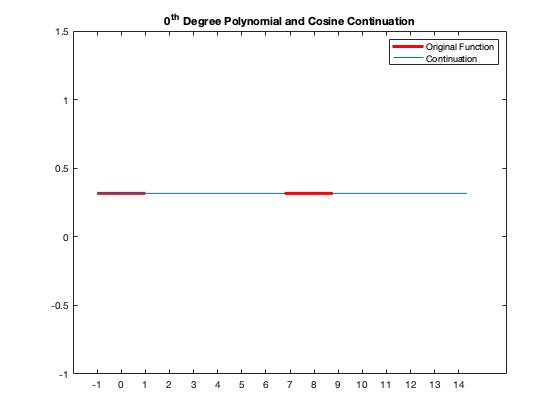
\includegraphics[scale=0.5]{ZeroDegreeCosineContinuation.jpg}
\caption{default}
\label{default}



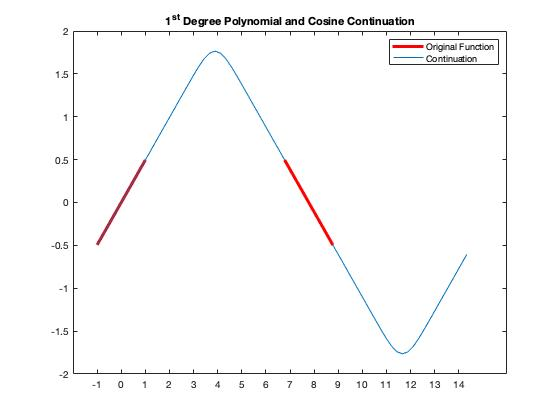
\includegraphics[scale=0.5]{FirstDegreeContinuation.jpg}
\caption{default}
\label{default}



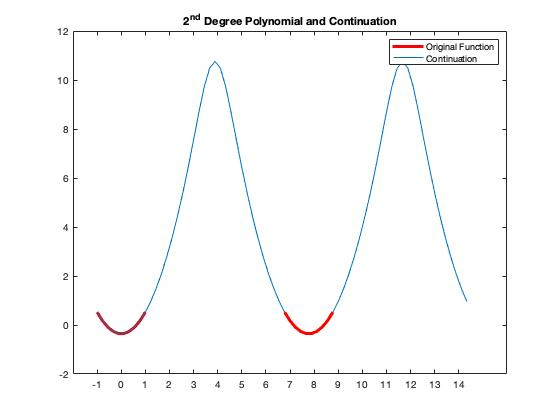
\includegraphics[scale=0.5]{SecondDegreeContinuation.jpg}
\caption{default}
\label{default}



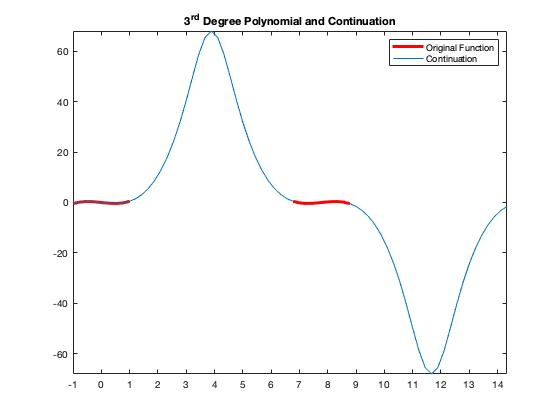
\includegraphics[scale=0.5]{ThirdDegreeContinuation.jpg}
\caption{default}
\label{default}



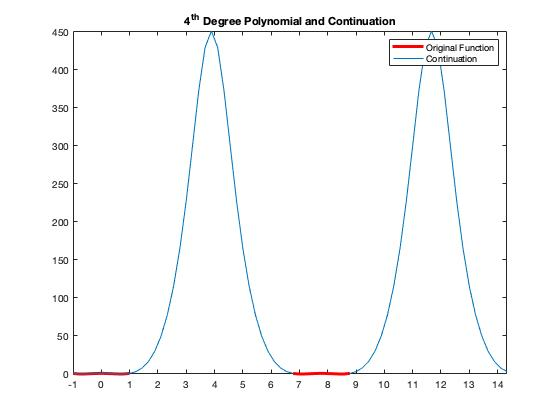
\includegraphics[scale=0.5]{FourthDegreeContinuation.jpg}
\caption{default}
\label{default}

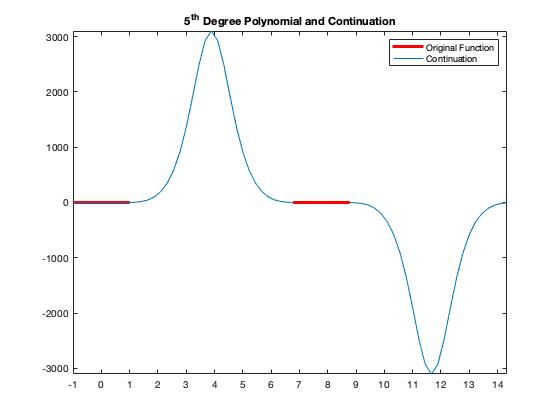
\includegraphics[scale=0.5]{FifthDegreeContinuation.jpg}
\caption{default}
\label{default}



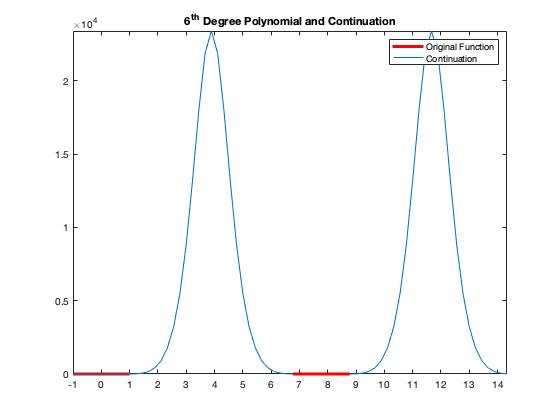
\includegraphics[scale=0.5]{SixthDegreeContinuation.jpg}
\caption{default}
\label{default}



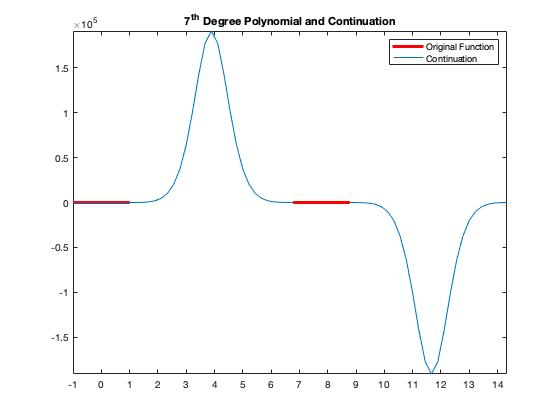
\includegraphics[scale=0.5]{SeventhDegreeContinuation.jpg}
\caption{default}
\label{default}


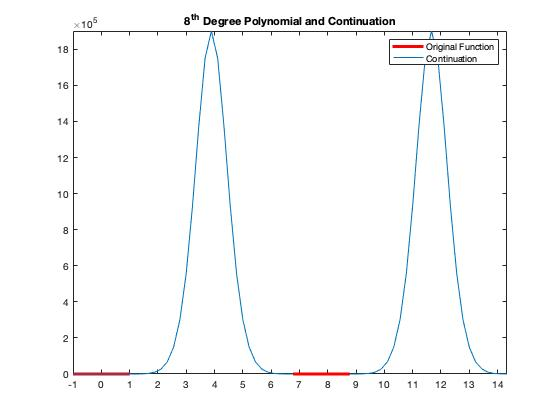
\includegraphics[scale=0.5]{EightDegreeContinuation.jpg}
\caption{default}
\label{default}



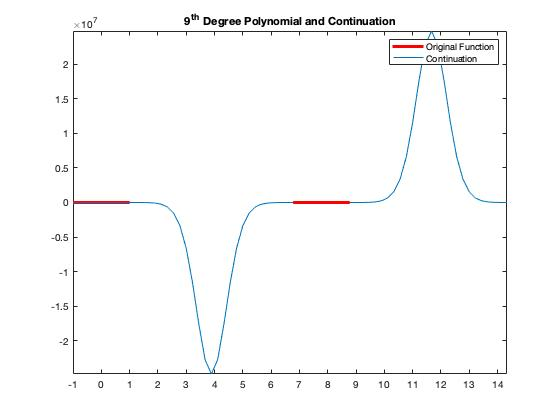
\includegraphics[scale=0.5]{NinthDegreeContinuation.jpg}
\caption{default}
\label{default}


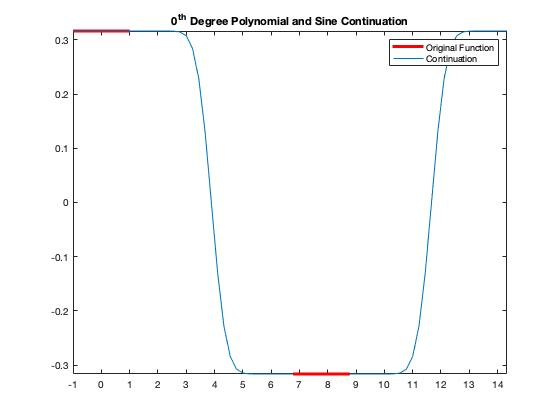
\includegraphics[scale=0.5]{ZeroDegreeSineCont.jpg}
\caption{default}
\label{default}




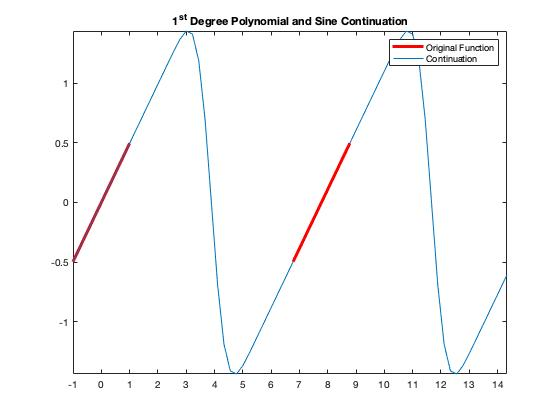
\includegraphics[scale=0.5]{FirstDegreeSineCont.jpg}
\caption{default}
\label{default}



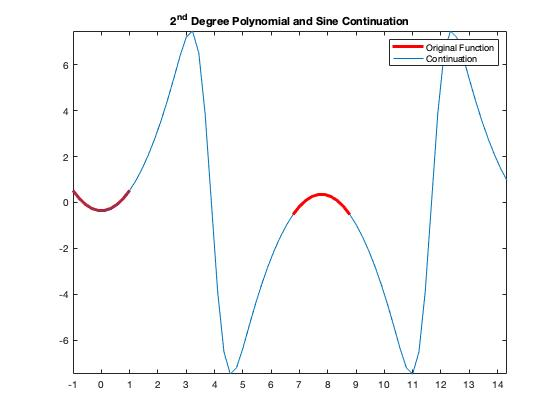
\includegraphics[scale=0.5]{SecondDegreeSinCont.jpg}
\caption{default}
\label{default}



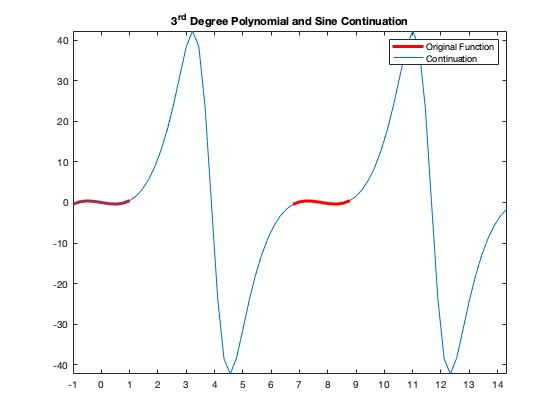
\includegraphics[scale=0.5]{ThirdDegreeSineCont.jpg}
\caption{default}
\label{default}




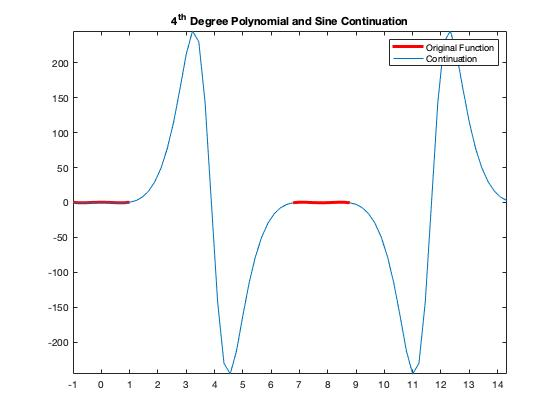
\includegraphics[scale=0.5]{FourthDegreeSineCont.jpg}
\caption{default}
\label{default}


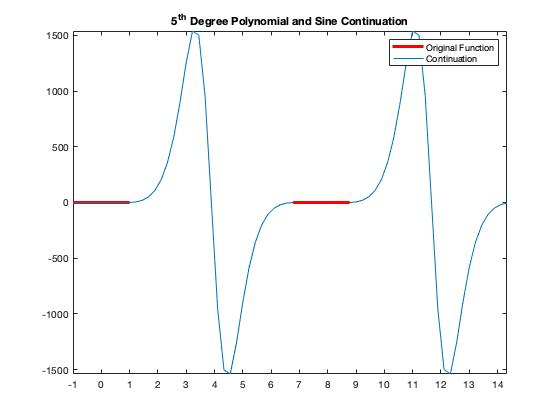
\includegraphics[scale=0.5]{FifthDegreeSineCont.jpg}
\caption{default}
\label{default}


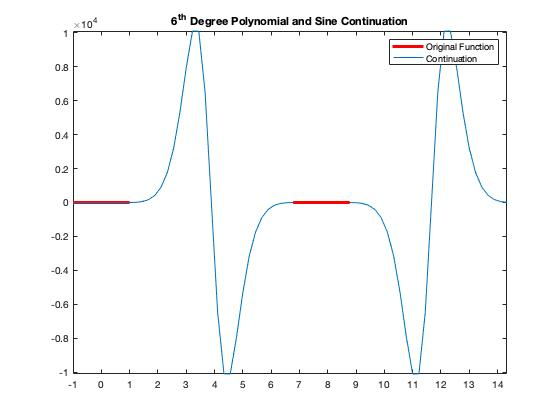
\includegraphics[scale=0.5]{SixthDegreeSineCont.jpg}
\caption{default}
\label{default}




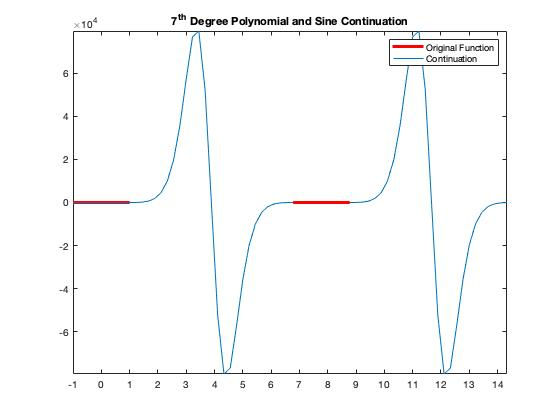
\includegraphics[scale=0.5]{SeventhDegreeSineCont.jpg}
\caption{default}
\label{default}
\end{center}
\end{figure}




\subsection{Accuracy of FC-approximations} FC-Gram approximations are a fast, accurate way to approximate functions using Fourier Continuation methods.  There are two main restrictions on the accuracy of the approximations. The limit to the accuracy of FC-Gram is how well the needed points can be approximated by the Gram polynomials. Even assuming the FC-Gram method were a perfect match, the accuracy would still be hindered by this function approximation. The function approximation can be made using QR-Factorization, and the accuracy is limited by the conditioning of that system.  However, in practice, this issue is only found when here is a lot of random noise at the ends of the sampled function.  With FC-Gram, since the method only requires the first $n$ points and the last $n$ points to be used for the approximation, if the function is even somewhat well-behaved at the ends, the first and last $n$ points of the functions will be easily approximated with low-degree polynomials, resulting in a high-accuracy approximation in that step.   \\ \\
Next, we focus on the accuracy of the Fourier Continuation approximation itself.  In [Lyon 2012 Accuracy-cite here], it was shown that the error between a function approximated with a Fourier Continuation has an error on the order of the error of an FFT. . \\ \\
 Once the FC-Gram method is used to find a Fourier Continuation for the function, the FFT is taken.  That FFT is then padded to oversample the function at a rate ten times greater than the original.  Then the IFFT is taken and compared with the original function on the ten times finer grid.  The $N$ is given as the original, coarse grid number of points and not the fine grid. To calculate the error, let $f^C$ be the computed continuation (using the FC-Gram method). Then $\mathscr{F}(f^C)$ is the FFT of the continuation.  Padding the FFT with zeros, so that its size is 10 times larger (arbitrarily chosen, but oversampled enough that it should pick up any error that could come from the sampling rate) gives $\mathscr{F}_P(f^C)$.  Taking the appropriately-scaled IFFT yields a result in the original domain, on a 10-times finer grid: $\mathscr{F}^{-1}(\mathscr{F}_P(f^C))$.  The original function is calculated on the finer grid, $x_F$.  The error is calculated as

\begin{equation}
E_{FCG}=\max_{x_F \in [-1,1]} |f(x_F)-\mathscr{F}^{-1}(\mathscr{F}_P(f^C))|
\end{equation}



As an example, when the FC-Gram method is applied to the function $f(x)=e^x$ on the interval $[-1,1]$, so chosen because of its lack of symmetry at the ends, we see excellent convergence (see Figure \ref{figure:FCExp}. 
\begin{figure}[h]
\begin{center}
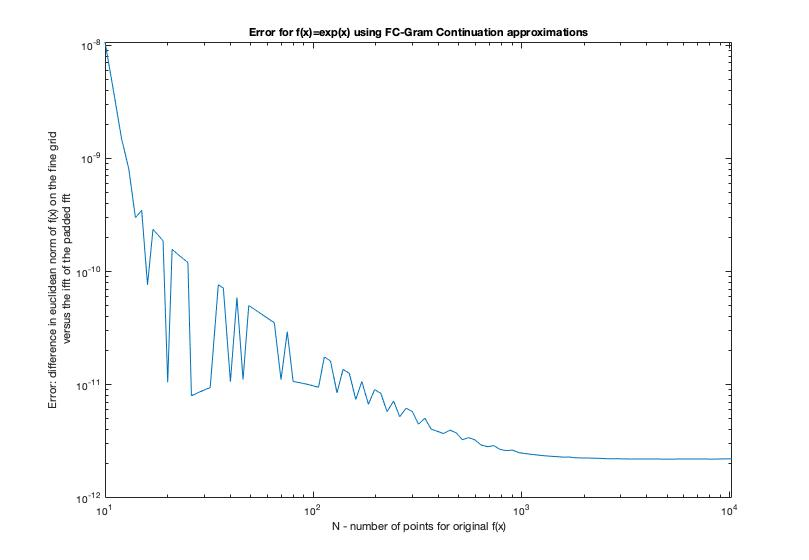
\includegraphics[scale=0.5]{ErrorFCGramonExp.jpg}
\label{figure:FCExp}
\end{center}
\end{figure}
Note that this is considered to be a ``worst-case" scenario for the FC-Gram method for a few reasons: as described above, the exponential function lacks symmetry at the endpoints making the left and right approximations different (i.e. the coefficients will have different complexity in their calculation and are not anticipated to be the same). In addition, the exponential function is very difficult to approximate with periodic functions from the start - regardless of the number of Fourier modes chosen in an approximation \textbf{cite Huybrechs and Adcock paper} \\ 

One can also consider the Runge function $f(x)=\frac{1}{1+25x^2}$, which is the most cited example of how accuracy can fall apart when trying to approximate a function on an increasing number of equispaced points.  In fact, the Runge function is a better candidate for the FC-Gram method because of its symmetry, but of course concern could be raised about how it will behave when increasing the number of points used in the approximation. However, because the FC-Gram method samples the first and last $N$ points and only approximates the function in those locations, the error does not increase as $N$ increases, and in fact, it behaves in quite the opposite manner. 

\begin{figure}[h]
\begin{center}
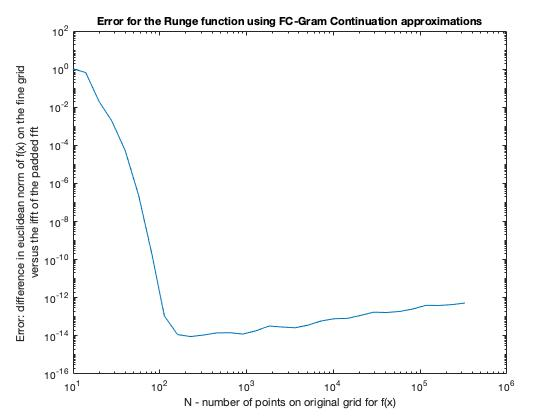
\includegraphics[scale=0.5]{ErrorRunge.jpg}
\end{center}
\end{figure}


\subsubsection{The FC-AD method}

The Fourier-Continuation Alternating-Direction algorithm is a method that applies the concept of Alternating Direction Implicit (ADI) methods to using a Fourier Continuation (FC) method in the spatial domain.  ADI methods reduce the numerical solution to PDEs into implicit first order boundary value problems in space.  In traditional ADI methods, these  BVPs are solved using finite-difference methods and yield low-accuracy results, particularly on the boundaries.  \\
Given the heat equation in two dimensions:
\begin{eqnarray}
u_t=k(u_{xx}+u_{yy}) + Q(x,y,t), & (x,y,t) \in \Omega \times (0,T], \nonumber \\
u(x,y,t) = G(x,y,t) & (x,y) \in \partial \Omega, t \in (0,T] \\
u(x,y,0)=u_0(x,y), & (x,y) \in \Omega, \nonumber 
\end{eqnarray}
with $k>0$, $\Omega \subset \mathbb{R}^2$ is smoothly bounded, and $Q$, $G$, and $u_0$ are smooth.  Discretizing according to $t^n=n\Delta t$, we then use a central difference scheme for the time derivative and enforce at $t^{n+\frac{1}{2}}=(n+\frac{1}{2})\Delta t$, resulting in
\begin{equation}
\dfrac{u^{n+1}-u^n}{\Delta t} = \dfrac{k}{2}\dfrac{\partial^2}{\partial x^2}(u^{n+1}-u^n) +\dfrac{k}{2}\dfrac{\partial^2}{\partial y^2}(u^{n+1}-u^n) + Q^{n+\frac{1}{2}} + E_1(x,y,\Delta t)
\end{equation}.
Here, $Q^{n+\frac{1}{2}}= Q(x,y,(n+\frac{1}{2})\Delta t)$ and $E_1(x,y,\Delta t)$ is the error term resulting from the central difference differentiation.  
Rearranging this equation yields
\begin{equation}
\left(1-\dfrac{k\Delta t}{2}\dfrac{\partial ^2 }{\partial x ^2 } - \dfrac{k\Delta t}{2}\dfrac{\partial ^2 }{\partial y ^2 }\right)u^{n+1}= \left(1+\dfrac{k\Delta t}{2}\dfrac{\partial ^2 }{\partial x ^2 } + \dfrac{k\Delta t}{2}\dfrac{\partial ^2 }{\partial y ^2 }\right)u^n + Q^{n+\frac{1}{2}}+E_1(x,y,\Delta t)
\end{equation}
and then factoring the left hand side and moving extra terms over gives 

\begin{equation}
\begin{aligned}
\left(1-\dfrac{k\Delta t}{2}\dfrac{\partial ^2}{\partial x^2} \right) \left(1-\dfrac{k\Delta t}{2}\dfrac{\partial ^2}{\partial y^2} \right)u^{n+1}& =  
\left(1+\dfrac{k\Delta t}{2}\dfrac{\partial ^2}{\partial x^2} \right) \left(1+\dfrac{k\Delta t}{2}\dfrac{\partial ^2}{\partial y^2} \right)u^n\\ &+ \dfrac{k^2 \Delta t^2}{4}\dfrac{\partial ^ 2}{\partial x^2}\dfrac{\partial ^2}{\partial y ^ 2} (u^{n+1}-u^n) + \Delta t Q^{n + \frac{1}{2}} + \Delta t E_1(x,y,\Delta t)
\end{aligned}
\end{equation}.

To solve for $u^{n+1}$, the operators on the left side must be inverted, which results in equations of the form 
\begin{eqnarray} \label{DiffEq}
u-\alpha u'' = f, & u(x_{\ell})=B_{\ell}, & u(x_r)=B_r 
\end{eqnarray}
where $\alpha=\dfrac{k\Delta t}{2}$ \cite{FCAD1}.  This turns a 2-D Partial Differential Equation into a sequence of 1-D Boundary Value Problems, which can be solved via whichever method is chosen.  For the FC-AD method, a Fourier Continuation approximation is used to solve the differential equation numerically.  \\ 




\subsubsection{ODE Solutions using Fourier Continuations}
While the following analysis applies to any linear differential operator, the differential equation \ref{DiffEq} will be the focus as its application is of most interest to this dissertation.  
Equation \ref{DiffEq} can be rewritten as 
\begin{equation}
(1-\alpha \dfrac{d^2}{dx^2})u=f
\end{equation}
To solve using Fourier Continuations, first the equation is discretized on a given (assumed equispaced) grid: $f_j=f(x_j)$ for $j=1,\ldots n$ and the solution $u_j=u(x_j)$.  
The Fourier continuation is calculated for $f_j$.  Then the FFT is taken of both sides, thereby diagonalizing the differential operator, heretofore referred to as $D$, where 
\begin{equation}
D_{kk}=1+\alpha k^2
\end{equation}
for each of the modes $k$.  








\section{Stability of Fourier Continuation in ODE Solutions}
First and foremost, it cannot be assumed that using a Fourier Continuation approximation to solve an ODE will be stable if the operator itself isn't stable in a continuous space.  The differential equation \ref{DiffEq} subject to boundary conditions 
\begin{eqnarray*}
u(a)&=&0 \\ 
u(b)&=&0
\end{eqnarray*}
is stable.  This stability is measured based on the function $f$: given an input of $f$ such that $\|f\|=1$, the solution $u$ should be such that $\|u\| \leq 1$.  This can be shown using the Green's function form of the solution.   The Green's function itself, constructed from the homogenous solutions, is forced to agree with boundary conditions.  When measuring the $\infty$ norm of $u$ as $\sup_{x \in [-1,1]} u(x)$, this yields
\begin{eqnarray*}
\sup_{x \in [-1,1]} u(x) &=& \sup_{x \in [-1,1] } \int_{-1}^{1}G(x,a)f(a)da \\
 &=& \int_{-1}^{1} \sup_{x \in [-1,1]} G(x,a)f(a)da \\ 
 &\leq& \int_{-1}^{1} f(a)da \\
 &\leq & 1 
\end{eqnarray*}
with equivalencies drawn because the convolution integral for the Green's function converges, and because the construction of the Green's function guarantees that the Green's function itself must be 0 at the boundaries  and have at most a jump discontinuity of 1.  
Shown below are some of the analytical solutions using the Green's function applied to $f(x)$ where $\|f\|_{\inf}=1$ for various values of $\alpha$. It can be seen that for larger values of $\alpha$, the maximum value of the solution is significantly smaller. The focus of stability questions for the remainder of this dissertation loosely assume stability for large values of $\alpha$ and focus numerically on the smaller values of $\alpha$, for as the solution gets closer and closer to the original function (as $\alpha \to 0$), any numerical error introduced could amplify and push the solution to have a maximum value above 1.  
\begin{figure}[htbp]
\begin{center}
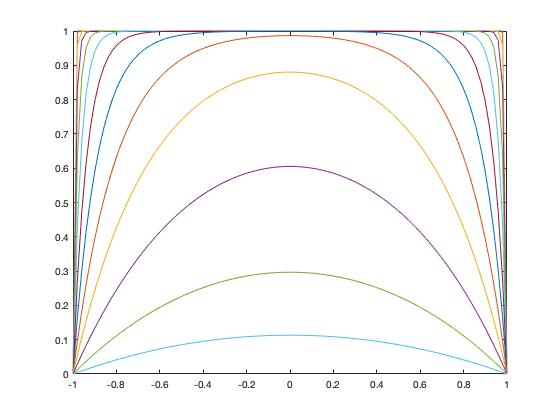
\includegraphics[scale=0.5]{Greens0.jpg}
\caption{G0}
\label{G0}
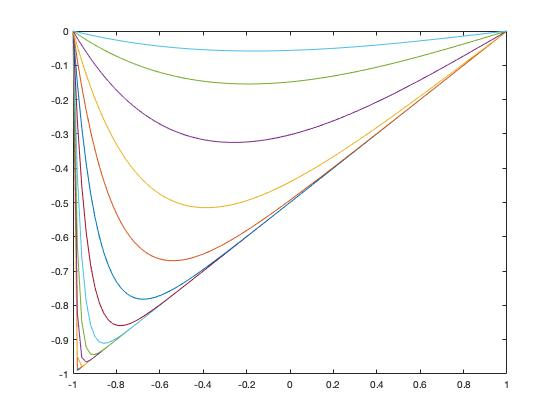
\includegraphics[scale=0.5]{Greens1.jpg}
\caption{G1}
\label{G1}
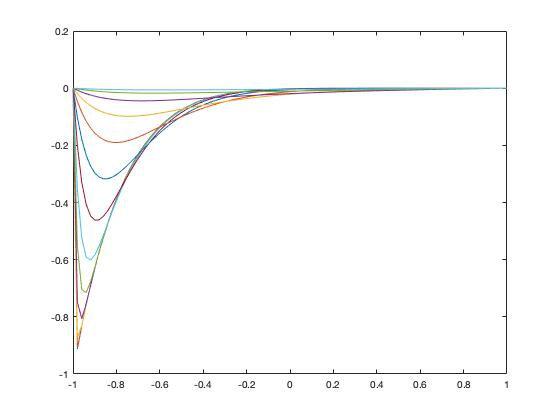
\includegraphics[scale=0.5]{Greens9.jpg}
\caption{G9}
\end{center}
\end{figure}



\subsection{Stability of FC-approximations}
Without applying any schemes, using the FC-Gram method to approximate the function $f$, and then using the properties of FFTs to solve differential equations like Equation \ref{DiffEq} yields accurate but occasionally unstable results.  \\
Stability is calculated by first using FC-Gram and FFTs to solve the differential equation with initial data $f=\mathbf{e}_i$, $i=1,\ldots n$. Note: the vectors $\mathbf{e}_i$ are the columns of the identity matrix $\mathbb{I}$. 
The solution $u_{\text{temp}}$ is calculated for each of the $\mathbb{e}_i$ and the homogeneous solutions are then applied, ideally removing as many ``un-reachable" frequencies as possible while enforcing boundary conditions.  
Then each solution $u_i$ is stored as a column in a matrix of solutions $U$, such that each column of $U$ corresponds to the same column of $\mathbb{I}$ of initial data. 
The stability is calculated by taking the SVD of the matrix $U$.  The singular values $S_{ii}$ of the SVD demonstrate any amplification of error that will take place.  If any $S_{ii}$ are greater than 1, the result is unstable.   
\\
Though this is the formal test of stability, along the way stability is tested for various choices of $f$ by calculating the corresponding solution $u$, enforcing boundary conditions through use of the homogeneous solutions, and then taking the ratio of the size of the solution to the size of the original function, or 
\begin{equation} 
s=\dfrac{||u||}{||f||}
\end{equation}
with $|| \cdot ||$ either representing the Euclidean (2-)norm or the max-norm.  


Without applying any scheme to the FC-Gram approximation process, and using the process described in the above section, the following stability results are achieved for a sample of $\alpha$ between $0.0001$ and $1$. 
\begin{figure}[htbp]
\begin{center}
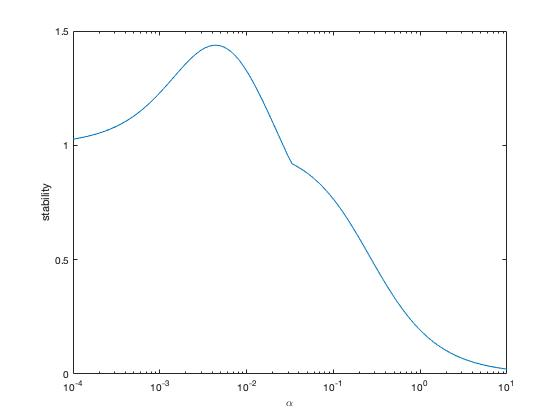
\includegraphics[scale=0.5]{StabilityGraphDeg0.jpg}
\caption{Stability of Fourier Continuations Under the Given Differential Operator with No Changes}
\label{Stab1}
\end{center}  
\end{figure}
As shown in Figure \ref{Stab1}, while for some larger values of $\alpha$ and some smaller values of $\alpha$ there is inherent stability in the system. While it would be excellent to just ignore the range of $\alpha$ values for which the system is unstable, that would not be practical in application as the time-stepping could lead to any possible value of $\alpha$.  
This change of behavior from the analytic must be contributed to not the behavior of the forcing function $f$ inside the domain in question but to the shape of the continuation outside of the original domain (in the extended domain).  As a general approximation scheme, without use as a differential operator solver, the shape of the continuation does not affect accuracy results (that is, the continuation could take on several different shapes in the extended domain and the accuracy should not be affected).  However, because of the ``smoothing" property that the second-derivative operator takes on, large values of the continuation in the extended domain can get smoothed back into the original domain as the operator is applied, thus introducing potential instability into the solution.

The three schemes proposed in this dissertation provide alternative stabilization schemes that rely on a priori changes to the continuation matrix, before applying the FC-Gram method. These changes suggest that controlling the behavior of the continuation outside the original domain will affect the stability of the approximation.  \\
The first scheme attempts to modify the shape of the continuation by forcing the continuation itself to match the function as usual, but adding an additional constraint that the application of the pseudo-inverse of the differential operator to the function must match the Green's function solution, discretized on the given domain. \\
The second scheme looks at the underlying mechanics of inverting the continuation matrix, and uses the SVD of the continuation matrix to try to minimize the changes made, while still focusing on accuracy and leveraging another constraint to keeping the continuation small in the extended domain.  \\
The final scheme attempts to only remove pieces of the continuation that contribute to the instability through brute-force calculations. 





\subsection{Error Approximation and Tolerances}
%
%
%
\subsubsection{Establishing Error Results}
When approximating a function $f$ using an orthogonal set of $n$ polynomials $\Phi_0$, $\Phi_1$, $\ldots$, $\Phi_{n-1}$ , we expect the error between the function $f$ and its approximation $\hat{f}$ to behave like
\begin{equation}
||f-\hat{f}|| = h^0 E_0 + h^1 E_1 + \ldots + h^{n-1} E_{n-1},
\end{equation} 
where $E_0$-$E_{n-1}$ are defined as $||\Phi_i-\hat{\Phi}_i||$ and are known, and the value of $h$ is determined by the accuracy desired. 
Assuming the highest degree polynomial will have the largest error, $h^{n-1}E_{n-1}$ can be used to find the value of $h$. 
(For example, if using a set of $n=10$ orthogonal polynomials, with an error $E_9=1e-2$, if 16 digits of accuracy are desired for the approximation of $f$, $h^9 E_9  = 1e-16$, giving us $h^9=1e-14$ or $h\approx 3e-2$.  Using this, in order to maintain an accuracy of 1e-16, for the 4th degree polynomial the term $h^4E_4$ must also equal $1e-16$, so $E_4$ must be approximately $1e-10$).  \\Operating within these bounds, it can be seen that high accuracy is needed in the lower degree polynomials, but that higher accuracy in the higher degree polynomials will not affect the overall accuracy of the approximation.  \\
Thus, instead of enforcing a strict machine-precision tolerance to approximate each polynomial, the tolerance is relaxed.  This appears in the SVD solve of the system of equations.  By relaxing the tolerance, some of the high-frequency modes which would cause the continuations to grow larger over a shorter interval are taken out of the system.  This controls the size of the continuations and allows for the transition from high precision to double precision without loss of accuracy. 
\subsection{Trade-Off of Stability and Accuracy}
There is a definitive trade-off in stability of the differential operator solution and the accuracy of the continuation as it matches the function.  The more stable, the less accuracy is seen overall. In order to keep the FC-AD scheme at the same order of accuracy overall, we want the scheme to be as accurate as possible, but without stabilization, the scheme can introduce significant errors that will propagate each time step. Using error approximation to guide the desired accuracy of the results allows us to enforce stability with the higher-degree polynomials while relaxing the error tolerance for what would be considered an 	``acceptable" approximation.  The trade-off in accuracy and stability will be shown in each scheme as it is the most important factor when we want a high-order accurate and stable method. 



\section{First Method: Matching Green's Functions}
\subsubsection{Green's Functions}
The Green's Function solution was then calculated via the methods described in Bender and Orszag: Let 
\begin{equation}
G(x,a)=\begin{cases}
A_1(a)h_1(x)+B_1(a)h_2(x) & x<a \\
A_2(a)h_1(x)+B_2(a)h_2(x) & x \geq a
\end{cases}
\end{equation}
where $h_1(x)$ and $h_2(x)$ are the homogeneous solutions to  $(I-\alpha \frac{\partial^2}{\partial x^2})u=f$:

\begin{eqnarray}
h_1(x) &=& e^{\frac{(x-b)}{\sqrt{\alpha}}} \\
h_2(x) &=& e^{\frac{(-x-1)}{\sqrt{\alpha}}},
\end{eqnarray}

where $h_1$ and $h_2$ have been normalized to $1$ on the boundary.  $A_1$,$A_2$,$B_1$, and $B_2$ are computed to enforce continuity of the Green's Function, at most a small jump discontinuity of the Green's Function, and zero boundary conditions \cite{BO}.  The Green's Function for our BVP ends up being

\begin{equation}
G(x,a)=\begin{cases} 
-\dfrac{1}{2} \dfrac{\sqrt{\alpha}\left(-e^{\frac{-1-2b+a}{\sqrt{\alpha}}}+e^{-\frac{a+1}{\sqrt{\alpha}}}\right)\left(-e^{\frac{2(2+b+x)}{\sqrt{\alpha}}}+e^{\frac{2(x+1)}{\sqrt{\alpha}}}+e^{\frac{2(1+b)}{\sqrt{\alpha}}}-1\right)e^{\frac{-x+1+2b}{\sqrt{\alpha}}}}{\left(e^{\frac{2(1+b)}{\sqrt{\alpha}}}-1\right)^2} & x<a \\
\dfrac{1}{2} \dfrac{\sqrt{\alpha} \left(e^{\frac{2+b+a}{\sqrt{\alpha}}} -e^{\frac{a-b}{\sqrt{\alpha}}}\right)\left(e^{\frac{2(-x+b)}{\sqrt{\alpha}}}+e^{\frac{2(1+b)}{\sqrt{\alpha}}}-e^{\frac{2+4b-2x}{\sqrt{\alpha}}}-1\right)e^{\frac{2+b+x}{\sqrt{\alpha}}}}{\left(e^{\frac{2(1+p)}{\sqrt{\alpha}}}-1\right)^2} & x \geq a

\end{cases}
\end{equation}

The final calculation of the Green's Function solution to the BVP comes from the convolution integral
\begin{equation}
u_G=\int_{-1}^b G(x,a)f(a)da.
\end{equation}
where $u_G(x)$ is the Green's Function solution for given $f(x)$.

\subsubsection{System of Equations}

Starting with $n$ points, the number of points desired on the coarse grid, and the minimal number of points needed to perform the FC-Gram computations, consider $x \in [-1, 1-\dfrac{2}{n}]$.  Splitting this interval into $n$ equispaced points gives us $\{x_j\}_{j=0}^9$.  We then compute the coefficients for the Gram Polynomials $f_0,f_1,\ldots f_9$(and their point values on the grid) by computing the QR factorization of the Vandermonde matrix of $\{x_j\}$.  While having the point values is enough if we were using a coarse grid, we need the coefficients of the polynomials both to compute the point values on a fine grid and also to compute the Green's Function solution.  


A finer grid is also constructed, $\tilde{x}$.  We choose the fine grid to be $F$ times more refined than the coarse grid, giving $h_f=\dfrac{h}{F}$.  Using the coefficients, the Gram Polynomials were calculated first as symbolic expressions, and then evaluated on the fine grid, giving  $\tilde{f}_0,\tilde{f}_1,\ldots \tilde{f}_9 $.  also construct the homogeneous solutions, $h_1(x)$ and $h_2(x)$, and evaluate them on the fine grid, giving us $\tilde{h}_1$ and $\tilde{h}_2$.  

Next, the Green's Function solution is computed for the given Gram Polynomial and the solution is evaluated on the fine grid. The Green's Function solutions for the monomials were computed symbolically using Maple and the expressions for these solutions were stored.  Using the linearity of integration, the Green's Function solutions were multiplied by the coefficients of the Gram Polynomials and added together,  then  the expressions were evaluated on $\tilde{x}$.  The evaluated Green's Function solutions are labelled  $\tilde{G}_0,\tilde{G}_1,\ldots,\tilde{G}_9$.  Here, $\tilde{G}_j$ depends both on the degree of the polynomial used and on $\alpha$. 

Next we compute the Fourier Continuation matrix.  In our first attempt we used complex exponentials (i.e. we constructed an $n \times n$ Discrete Fourier Transform matrix from $0$ to $2\pi$), however, because of the ill-conditioning of the system, error propagation ruined the preservation of even and odd modes depending on our desire for an even or odd continuation.  

To compute our Continuation Matrix, we start with our desire to have period $B$ (i.e. a period of $B$ times the original length). For our coarse grid, we use $n$ points on an interval of length 1, giving us step size $h_c=\dfrac{1}{n-1}$.  To continue this,  there will be  
\begin{equation}
L_d=(n-1)\times B \times 2
\end{equation}
 points for a double period continuation - one of the boundary points will not be included as it will be repeated.  The stability for the result is calculated on the coarse grid, so the number of points on the coarse grid gives a constraint for the number of modes we are able to use.  We choose to use 
 \begin{equation}
 M=\begin{cases}
 \texttt{floor}(\frac{L_d}{2}-1), & \text{Cosine} \\
 \texttt{floor}(\frac{L_d}{2}-2), & \text{Sine}
 \end{cases}
 \end{equation}
 modes for our expansions, noting that the cosine expansion includes the 0 mode, which is a little less than half the total number of coarse grid points used. 

We construct a fine grid of step size $h_f=\dfrac{h_c}{F}$ ($F$ times more refined than the original coarse grid) and get 
\begin{equation}
F_u=(n-1)\times F + 1
\end{equation} points on the unit length interval and 
\begin{equation}
F_e=(n-1)\times F \times B \times 2
\end{equation} points on our full double period interval (again, we don't include the very last point on the interval as it will get repeated). 

A discrete cosine transform (DCT) matrix is constructed on the fine grid over both the unit interval and on the extended interval, called $C_u$ and $C_e$ respectively.  $C_u$ should have $F_u$ rows and $M$ columns and $C_e$ should have $F_e$ rows and $M$ columns.  Similarly, we construct a discrete sine transform (DST) matrix on both the unite and extended fine grids, and call them $S_u$ and $S_e$ respectively, whose dimensions will be $F_u \times M$ and $F_e \times M$ for the appropriate $M$-value for sine.  It should be noted that both matrices operate from the space of modes and transform into point values.   

We now have a matrix  which we can use to express any function on the correct interval in terms of either a sine or cosine series with period $B$ over $M$ modes.  

Trying to create the cosine continuation for $f$ is the equivalent of solving
\begin{equation}
\min ||C_u f^c - \tilde{f} ||^2 .
\end{equation}
This would yield the coefficients $f^c$ for the Fourier Continuation approximation for $\tilde{f}$.  However, due to the unreliability of the system in terms of stability, additional constraints must be applied.  

This is where we diverge from previous literature.  Instead of experimenting numerically or pre-conditioning our data, instead the Green's function solution is used to hopefully constrain the system in order get a continuation that is stable under the given operator.  

From the differential operator of the BVP, a numerical differential operator can be constructed to represent $I-\alpha \dfrac{\partial ^2 }{\partial x^2}$ for both the sine and cosine transforms, noting that two different differential operators are used due to the difference in number of modes used for sine and cosine, $D_c$ and $D_s$. Then the inverted differential operator is applied to the Fourier Continuation coefficients, and then evaluated on point values using the continuation matrices. This is forced to match the point values of the Green's Function solution.

This adds a new constraint to our problem: 
\begin{equation}
\min ||C_u f^c - \tilde{f}|| ^2 + ||C_u D_c^{\dagger} f^c - \tilde{G}||^2
\end{equation} 

In this computation, it was discovered that the homogeneous solutions are not well-represented in terms of the cosine or sine basis, so the pieces of the homogeneous solutions that contribute to the Green's function solution will not be reached in solving this system, giving rise to high inaccuracy and also pulling away from the desired stability. To remedy this, the inverted differential operator is allowed to be modified by some linear combination of the homogeneous solutions.  This gives additional degrees of freedom to the system and also attempts to remove the dependence of the Green's function on functions that can't be represented in the Fourier bases.  

The system then becomes
\begin{equation}
\min ||C_u f^c - \tilde{f}|| ^2 + ||C_u D_c^{\dagger} f^c +c_1 \tilde{h_1} + c_2 \tilde{h_2} - \tilde{G}||^2
\end{equation}
where the constants $c_1$, $c_2$ are freely chosen by whichever algorithm is used to solve the system.  We use the SVD, which will minimize all of the coefficients it solves for, so we expect $c_1$ and $c_2$ to be (relatively) small.  


Adding this gives rise to great accuracy for both $f^c$ and the solution $u^c$ and almost-stability.  Two more constraints were added to the system in order to achieve stability: first, a parameter $\lambda$ which helps the algorithm to choose smaller values for $c_1$ and $c_2$,  which in turn allows our system to minimize the coefficients $f^c$. To implement this, we let $\lambda c_1 \tilde{h_1} + \lambda c_2 \tilde{h_2} = \bar{0}$, or in our system:
\begin{equation}
\min ||C_u f^c - \tilde{f}|| ^2 + ||C_u D_c^{\dagger} f^c +c_1\tilde{h_1}+c_2\tilde{h_2}- \tilde{G}||^2 + \lambda^2|| c_1 \tilde{h_1} + c_2 \tilde{h_2} ||^2.
\end{equation}

Using $\lambda$ affects the accuracy slightly but gives stability for every polynomial, for any value of $\alpha$.  

Stability can also be enforced by means of another parameter $\mu$ which is applied strictly to the inverted differential operator, but only on points that match with the coarse grid (since stability is computed only on the coarse grid), and the final system to solve becomes
\begin{equation}
\min ||C_u f^c - \tilde{f}|| ^2 + ||C_u D_c^{\dagger} f^c +c_1\tilde{h_1}+c_2\tilde{h_2}- \tilde{G}||^2 + \lambda^2|| c_1 \tilde{h_1} + c_2 \tilde{h_2} ||^2 + \mu^2||C_u D_c^{\dagger}|{\text{\tiny{coarse}}}  ||^2
\end{equation}


\subsection{Implementation}
We chose to implement the solver in the Julia computing language.  This choice was made because Julia has a storage type \texttt{BigFloat} which allows for arbitrary precision as opposed to the double-precision (64-bit).  Setting the precision in Julia to 200 bits allows calculations to be performed with an accuracy of approximately $\mathcal{O}(10^{-77})$, so even losing digits due to round-off error in solving the system, still yields a very high-accuracy result.  Using Julia packages \texttt{LinearAlgebra}, \texttt{SymPy}, \texttt{GenericSVD} and several proprietary functions,  the system above was created and solved using a singular value decomposition and pseudoinverses with a tolerance of $10^{-40}$.  

The matrix used to solve the minimization problem is:
\begin{equation}
\begin{bmatrix}
C_u & \mathbf{0} & \mathbf{0}\\
C_u D_c^{\dagger} & \tilde{h_1} & \tilde{h_2} \\
\mathbf{0} & \lambda \tilde{h_1} & \lambda \tilde{h_2} \\
\mu C_u D_c^{\dagger}|_{\text{\tiny{coarse}}} & \mathbf{0} & \mathbf{0}
\end{bmatrix}
\begin{bmatrix}
f^c \\
c_1\\
c_2
\end{bmatrix}
= 
\begin{bmatrix}
\tilde{f} \\
\tilde{G}\\
\mathbf{0}\\
\mathbf{0}
\end{bmatrix}
\end{equation}.  

Using the psuedoinverse of this matrix with a tolerance of $1e-40$ gives enough accuracy despite having condition numbers $\mathcal{O}(10^{17})$.  

For the computations made, we chose $n=10$ and $B=3.5$, and tested values of $\alpha$ ranging from $0.001$ to $1$.  




\section{Second Method: Singular Value Decomposition of the Continuation Operator}
The second scheme developed relies on the singular value decomposition of the continuation operator. In order to construct the continuation, a least-squares problem is constructed, which in essence becomes 
\begin{equation}
C f^C=f
\end{equation}
and the $f^C$ is then used in conjunction with the differential operator 
\begin{equation}
Du=f
\end{equation}
with an end result solving for $u$ as
\begin{equation}
C^{\dag}D^{\dag}f^C=u
\end{equation}
On the original domain, $f^C \sim f$, to numerical tolerances and thus we can expect $\|f^C\| \leq 1$.  The inverted differential operator $D^{\dag}$ is a diagonal operator whose values are all less than or equal to 1.  Thus, any instability must come from the pseudoinverse of $C$.  
$C^{\dag}$ is constructed from the SVD of $C$, that is, if $C=USV^{T}$, then $C^{\dag}=U^{T}S^{\dag}V$.  $S^{\dag}$ is computed using a numerical tolerance - if $s_{ii}<\text{tol}$, $s^{\dag}_{ii}=0$ to avoid division by zero or near-zero issues. It is expected that $S$ will contain some zero or near-zero singular values. This represents the modes of the sine or cosine functions that are not as influential in the continuation (principle components analysis).  The other properties stem directly from the definition and construction of the SVD.  

\subsection{Perturbation of the SVD}
The concern becomes the effect that the rows of $V^T$ have on the Fourier coefficients.  The scheme developed is aimed to find and then minimize rows of $V$ that exhibit behavior not easily attained by the choice of modes for the Fourier Continuation, thus attempting to control the size of $V^Tf^C$, subject to the constraints of accuracy (that the changes to the continuation itself must retain a high level of accuracy) and size (that the size of the continuation must remain small enough to be usable).  
Thus we have the following minimization problem: 
\begin{eqnarray}
\text{minimize} & |CD^{\dag}V\gamma - C D^{\dag}f^C| \\
\text{and} & ||S|| \\
\text{subject to} & Cf^c = f
\end{eqnarray}
The goal is to find the ``problematic" columns of V, and use $\gamma$ to remove those values from the solution entirely, while keeping the size of the singular values small and maintaining accuracy of the continuation matrix. 
Removing a linear combination of the columns of V will change the shape of the continuation but as long as we keep the constraints in place the accuracy in the original domain should not be affected. 
\subsubsection{Stability for the Polynomials as a Function of $\alpha$}
%
%
%
\subsubsection{Interpolation}
%
%
%
\section{Third Method: Brute Force Modification of the Continuation in the Extended Domain}


\section{Conclusions and Future Work}
\subsection{Stability of Each Scheme}
\subsection{Accuracy of Each Scheme}
%
%
%

\end{document}

